% command to make sure colorboxes don't create whitespace between code lines
\fboxsep=.6pt

% default settings for listings
\lstset{style=python, basicstyle=\scriptsize\ttfamily}

\begin{frame}
    \centering
    \begin{figure}[H]
        \includegraphics[keepaspectratio, width=0.7\paperwidth, height=\paperheight]{\thelogo}
    \end{figure}
    Informatik: Programmieren\\
    \emoji{clipboard} Kapitel 5: \textbf{Listen (Teil 2)}
\end{frame}

\begin{frame}[fragile]{Beispiel: Tram}
Sie leiten die Entwicklung des Tram-Fahrplans in der Stadt Zürich. Die aktuelle Glatttalbahn (Tram 12) fährt von Stettbach, bzw. Oerlikon, bis zum Flughafen (s. folgende Abbildungen). Ignorieren Sie die blaue Linie, die bei ``Glattpark'' nach rechts abbiegt.
\end{frame}
\begin{frame}[fragile]{Beispiel: Tram}

\begin{figure}[H]
\centering
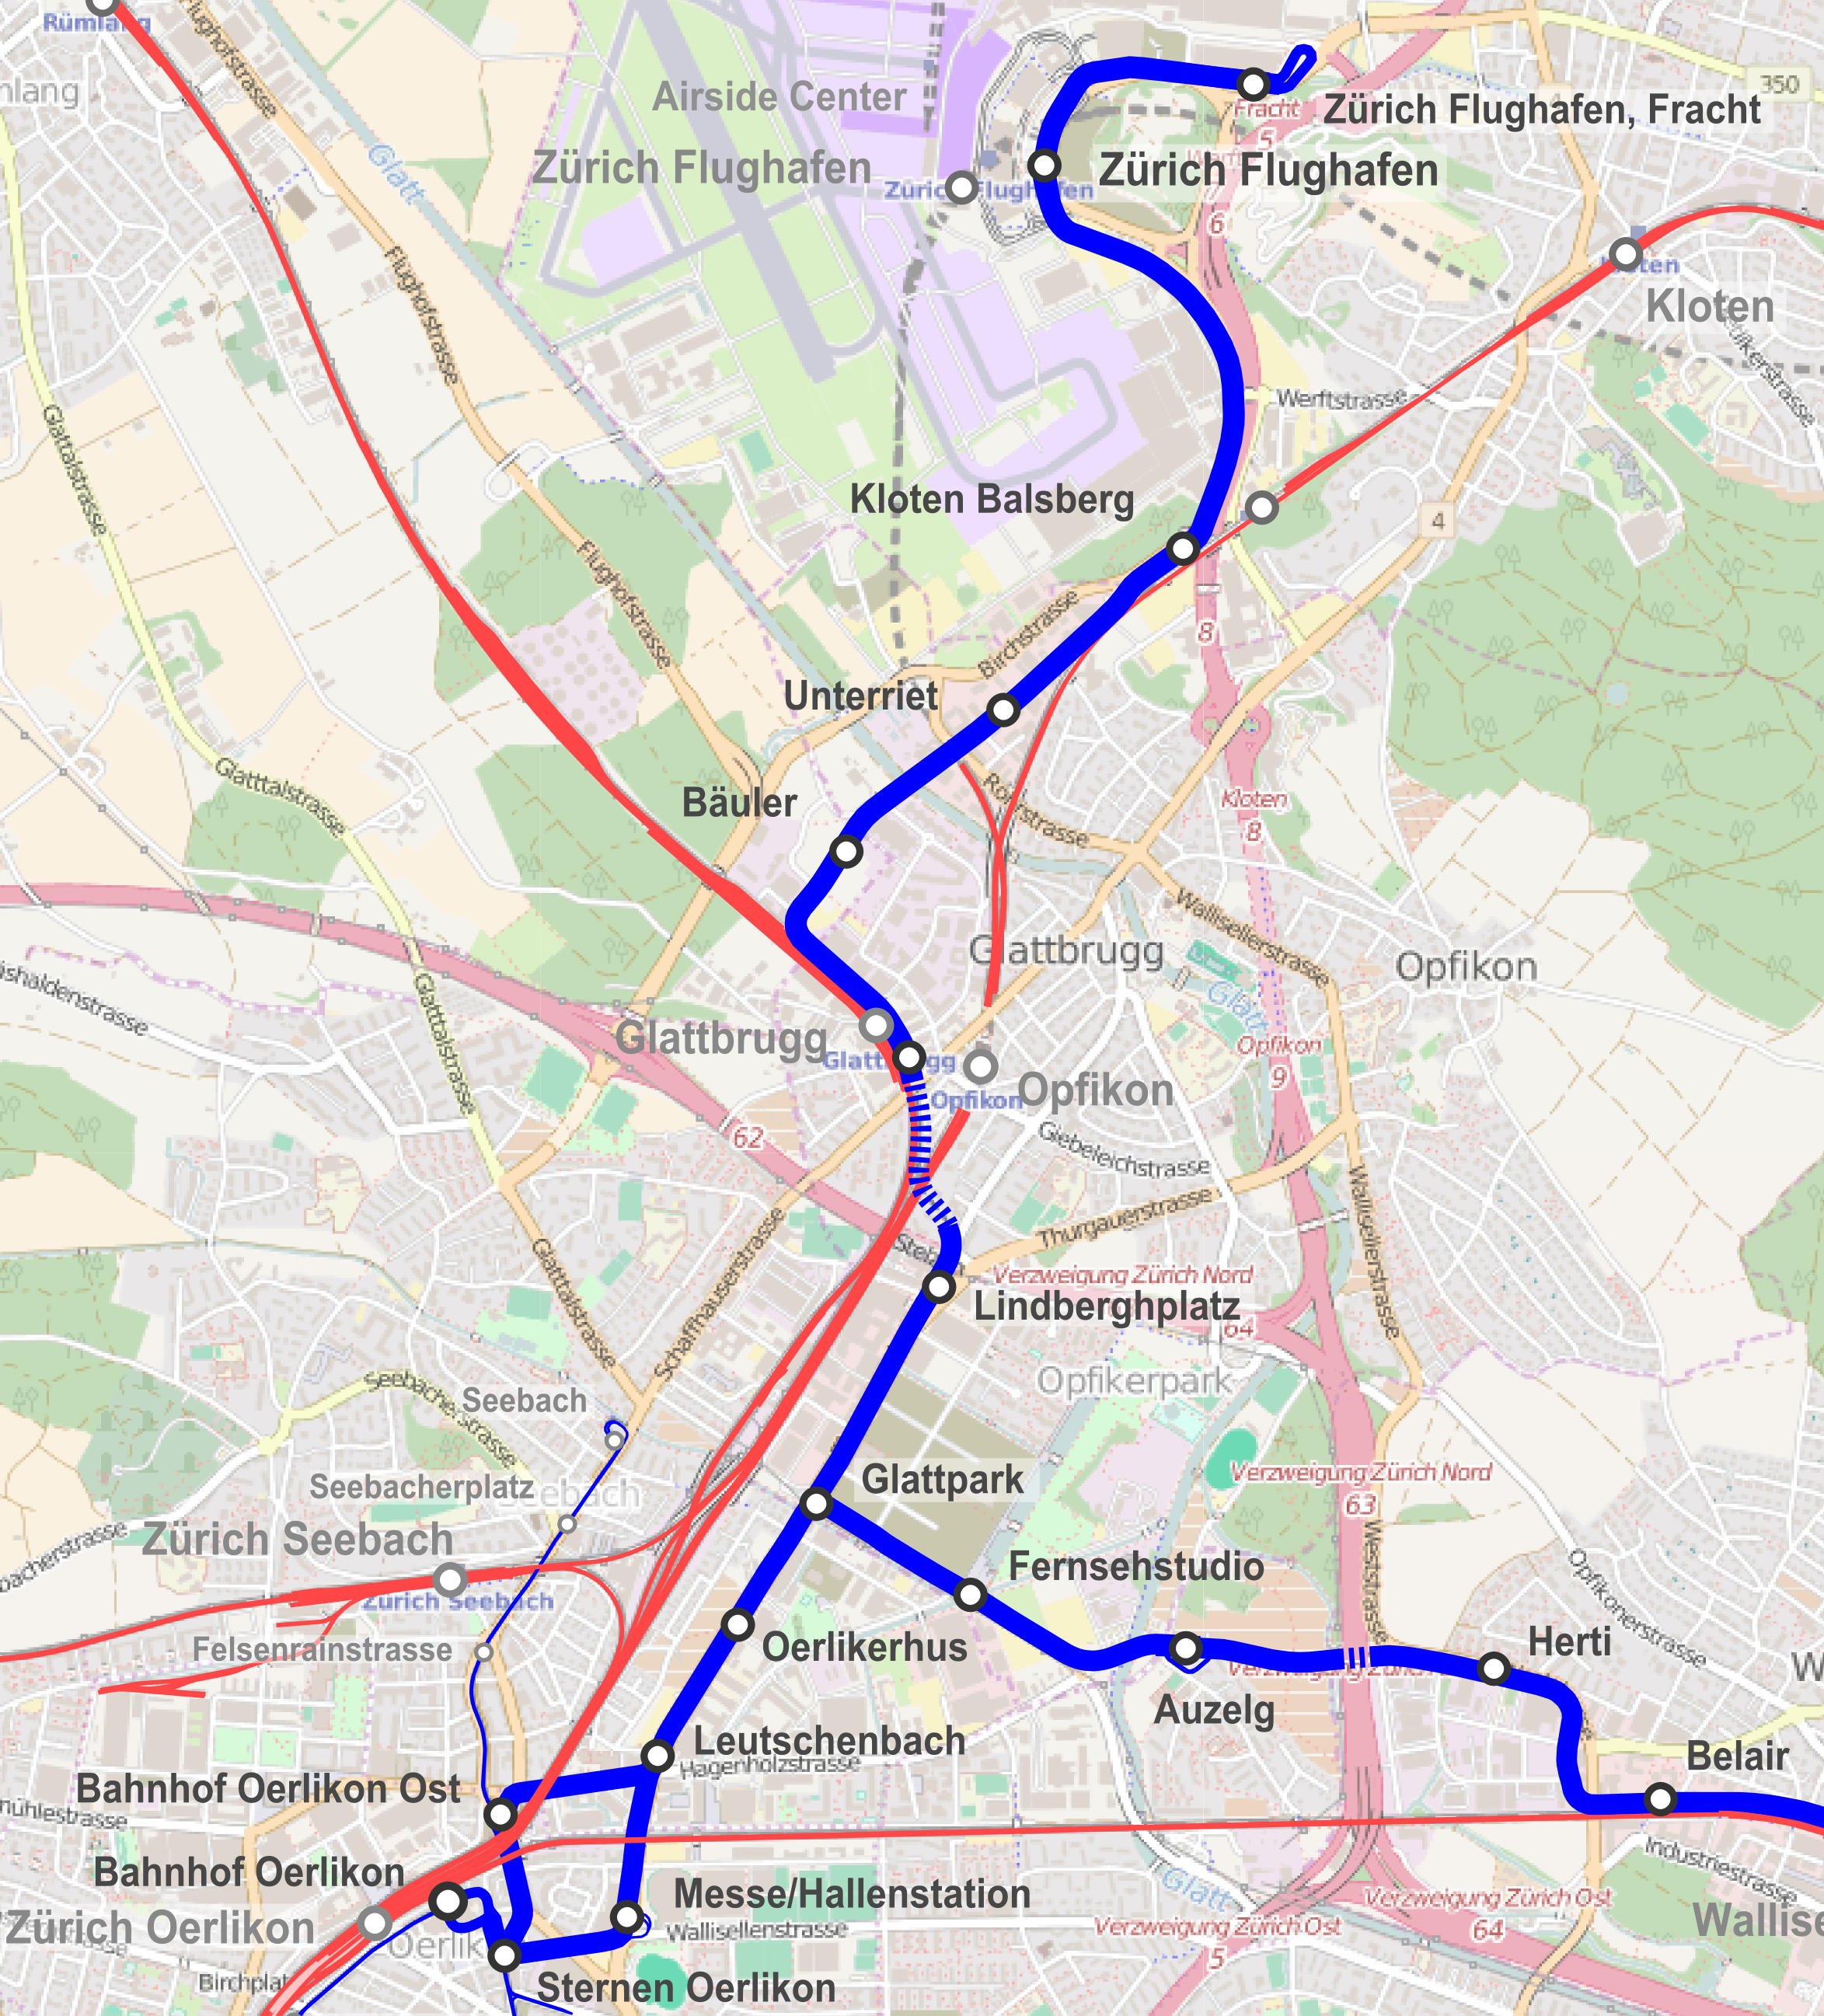
\includegraphics[width=.6\linewidth]{Grundlagen_Info/00_Programmieren/Figures/Glattalbahn_vbg}
\end{figure}

\end{frame}
\begin{frame}[fragile]{Beispiel: Tram}

Sie haben sich folgende Stationen und die Fahrzeit von der Anfangs-Station ``Sternen Oerlikon'' zu jeder folgenden Station bis und mit ``Zürich Flughafen Fracht'' in Sekunden notiert:

\begin{lstlisting}
stationen = ["Sternen", "Messe", "Leutschenbach", "Oerlikerhus", "Glattpark", "Lindbergh", "Glattbrugg", "Bäuler", "Unterriet", "Kloten", "Flughafen", "Flughafen Fracht"]
dauer = [0, 60, 122, 185, 241, 363, 543, 603, 666, 729, 786, 845]
\end{lstlisting}

Die Glattal-Tramlinie soll nun erweitert werden um die folgenden Stationen:
\end{frame}

\begin{frame}[fragile]{Beispiel: Tram}
\begin{figure}
\centering
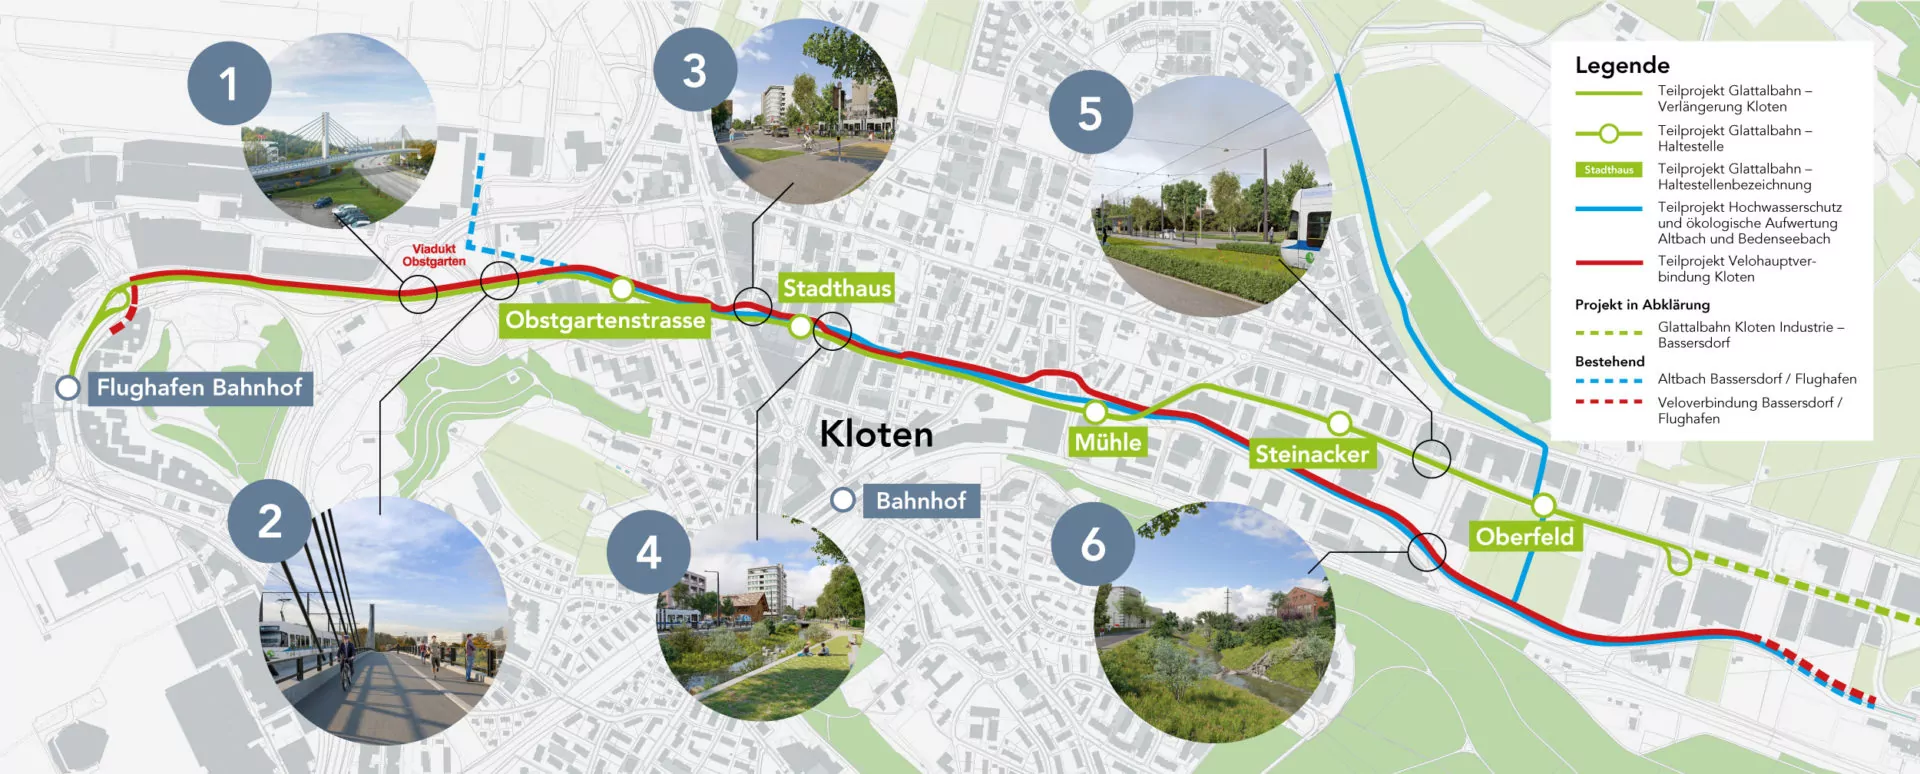
\includegraphics[width=\linewidth]{Grundlagen_Info/00_Programmieren/Figures/GTB_Karte_mit_Legende_Web_v02}
\end{figure}
Was könnten wir im Code ändern, falls wir die Liste erweitern wollen?
\end{frame}
    


\begin{frame}[fragile]{Datenstrukturen: Stapel \emoji{books}}
	\begin{itemize}
		\item \lstinline|meineliste.append(neu)|: Fügt ein Element \lstinline|neu| (einzelne Zahl oder Text) am Ende der Liste \lstinline|meineliste| hinzu
		\item \lstinline|meineliste.pop()|: Entfernt das letzte Element von \lstinline|meineliste|
	\end{itemize}
	\pause
	Beispiel:
	\begin{lstlisting}
	# stationen von vorher
	stationen = ["Sternen", "Messe", "Leutschenbach", "Oerlikerhus", "Glattpark", "Lindbergh", "Glattbrugg", "Bäuler", "Unterriet", "Kloten", "Flughafen", "Flughafen Fracht"]
	
	stationen.append("Obstgartenstrasse")
	stationen.append("Stadthaus")
	#...
	
	
	\end{lstlisting}
	\pause
	Einfacher:
	\begin{lstlisting}
	# stationen von vorher
	stationen = ["Sternen", "Messe", "Leutschenbach", "Oerlikerhus", "Glattpark", "Lindbergh", "Glattbrugg", "Bäuler", "Unterriet", "Kloten", "Flughafen", "Flughafen Fracht"]
	
	# liste an liste anhängen
	stationen += ["Obstgarten","Stadthaus","Mühle","Steinacker","Oberfeld"]
	\end{lstlisting}
\end{frame}

\begin{frame}[fragile]{Beispiel}
	\begin{lstlisting}
		zahlen = [3, 1, 7, -2, 6, -12, 5, 6, 9]
		weitere_zahl = input("Welche Zahl möchten Sie hinzufügen?")
		zahlen.append(weitere_zahl)
		print(zahlen) # Was wird gedruckt?
		
		zahlen.pop()
		zahlen.pop()
		print(zahlen) # Was wird gedruckt?
	\end{lstlisting}
\end{frame}

\begin{frame}[fragile]{Auf Listen zugreifen}{Von hinten}
Gegeben sei folgende Liste: \lstinline|x=[3, 10, 33, 2, 220, 11]|.\\

Wie können wir auf das letzte Element von \lstinline|x| (= die Zahl \lstinline|11|) zugreifen?
\begin{itemize}
\item \lstinline|x[len(x)-1]|
\item Einfacher: \lstinline|x[-1]|
\item Vorletztes Element: \lstinline|x[-2]|
\item Etc.
\end{itemize}
\end{frame}

\begin{frame}[fragile]{Fibonacci-Serie}
\begin{itemize}[<+->]
\item Was ist die Fortsetzung folgender Zahlen? 1, 1, 2, 3, 5, ...?
\item Wie würden wir einen Code dafür schreiben?
	\begin{lstlisting}
		fib = [1, 1]
for _ in range(100):
			# berechne nächste Zahl
			fib_neu = fib[-1] + fib[-2]
			fib.append(fib_neu)
		print(fib)
	\end{lstlisting}
\end{itemize}
\def\spiral#1{%
  \pgfmathparse{int(#1)}%
  \ifnum\pgfmathresult>0
    \draw [help lines] (0,0) rectangle ++(1,1);
    \begin{scope}[shift={(1,1)}, rotate=90, scale=1/1.6180339887]
      \spiral{#1-1}
    \end{scope}
    \draw [red] (0,0) arc (270:360:1);
  \fi
}

\begin{figure}[H]
\centering
\tikz[scale=2]{\spiral{12}}
\end{figure}
\end{frame}



\begin{frame}[fragile]{Auftrag}
	\begin{itemize}
		\item \aufgabebox{Aufgabe 5.18}
		\item \abgabebox{Aufgabe 5.19}
		\\[.1cm]$\rightarrow$ \textbf{Tipp}: Verwenden Sie \lstinline|daten[-1]|, um auf das letzte Element einer Liste \lstinline|daten| zuzugreifen, und \lstinline|daten[-2]| für das vorletzte Element.
		\item \abgabebox{Aufgabe 5.25}
		\item \aufgabebox{Aufgaben 5.21, 5.22, 5.23}
	\end{itemize}
\end{frame}


\begin{frame}[fragile]{Durch jedes Element in einer Liste durchgehen}{Flexibler Summen-Befehl (Möglichkeit 2/2)}
	\begin{lstlisting}
		def summiere(daten):
			summe = 0       # Variable, um alle Elemente von "daten" zu summieren
		
			# Durch alle Elemente von Daten durchgehen und zu Summe hinzufügen
			for d in daten:
				summe += d   # Wert zu Summe hinzufügen
		
			print(summe)
		
			daten = [4, 2, -6, 17, 5, 12] 
		summiere(daten)
	\end{lstlisting}
\end{frame}

\begin{frame}[fragile]{Durch jedes Element in einer Liste durchgehen}{Flexibler Summen-Befehl (Möglichkeit 2/2)}
	\begin{columns}
	\begin{column}{.5\textwidth}
	\begin{lstlisting}
def summiere(daten):
	summe = 0

	for d in daten:
		summe += d

	print(summe)

daten = [4, 2, -6, 17, 5, 12] 
summiere(daten)
		\end{lstlisting}
	\end{column}
	\begin{column}{.5\textwidth}
	\begin{lstlisting}
def summiere(daten):
	summe = 0
	index = 0
	
for _ in range(len(daten)):
		summe += daten[index]
		index += 1

	print(summe)

daten = [4, 2, -6, 17, 5, 12] 
summiere(daten)
		\end{lstlisting}
	\end{column}
	\end{columns}
\begin{itemize}[<+->]
	\item Die beiden obigen Codes sind identisch. Welchen bevorzugen Sie?
	\item \lstinline|d| nimmt jeden Wert von \lstinline|daten| genau einmal an
	\item \lstinline|d| ist eine Variable, man könnte den Namen also auch beliebig anders wählen
	\item \lstinline|d| ist also zuerst 4, dann 2, dann -6, etc.
	\item Die Schleife links wird ebenfalls 6 mal ausgeführt
\end{itemize}
\end{frame}

\begin{frame}[fragile]{Auftrag}
Im Buch
\begin{itemize}
	\item \aufgabebox{Aufgaben 5.30, 5.32}
	\item \readbox{Beispiel 5.12}
	\item \aufgabebox{Aufgabe 5.33}
	\item \abgabebox{Aufgabe 5.34}
	\item \aufgabebox{5.36 - 5.38}
	\item \readbox{Beispiel 5.14}
	\item \aufgabebox{5.39}
	\item \abgabebox{Aufgabe 5.41}
\end{itemize}
\end{frame}


\begin{frame}[fragile]{Appendix: Überprüfen, ob etwas in einer Liste ist}{Mani Matter (\href{https://youtu.be/gQbF9Ck1ccc?feature=shared}{Link})}
	
	\begin{lstlisting}
		zutaten_sandwich = ["brot", "fleisch", "anke", "brot"]
		
		if "brot" not in zutaten_sandwich:
			print("Was isch es Sandwich ohni Brot? S'isch nume Fleisch!")
		elif "fleisch" not in zutaten_sandwich:
			print("Was isch es Sandwich ohni Fleisch? S'isch nume Brot!")
		# usw. 
	\end{lstlisting}
\end{frame}

\begin{frame}[fragile]{Appendix: Überprüfen, an welcher Position in einer Liste ein Element ist}
	
\begin{lstlisting}
stationen = ["Bern", "Zürich", "Zürich Oerlikon", "Zürich Flughafen", "Winterthur", "St. Gallen"]
station = "Zürich Flughafen"
pos = stationen.index(station, 0, len(stationen))
print(pos) # Resultat ?
\end{lstlisting}
\end{frame}

\begin{frame}[fragile]{Auftrag}{\emoji{trophy} Challenge}
Auf Moodle, ``Zusatzaufgaben Listen \& Funktionen''
\begin{itemize}
	\item \challengebox{\emoji{tram} Fahrplan}
	\item \challengebox{\emoji{heart-with-arrow} Dating-App}
	\item \challengebox{\emoji{pirate-flag} Black-Friday-Rabatte}
\end{itemize}
\end{frame}